\chapter{Part}

\section{Model Estimation and Residual Diagnostics}

We split the data into a training set (January 1960 -- December 2015) and a test set (January 2016 - December 2019). As established in \ref{Question 1.4}, both models are estimated on the log-transformed series $\log(\text{CPI}_t)$, since differencing the original series revealed non-constant variance incompatible with ARIMA modelling.

The first model is selected by minimising AIC over a range of ARIMA specifications. The second is the model identified manually in \ref{Question 1.4}, ARIMA$(1,1,1)(0,1,1)_{12}$:
\[
(1 - \phi_1 B)(1 - B)(1 - B^{12})\log(\text{CPI}_t) =
(1 + \theta_1 B)(1 + \Theta_1 B^{12})\varepsilon_t
\]

where $B$ is the backshift operator, $\varepsilon_t \sim \text{WN}(0, \sigma^2)$,
$\phi_1$ is the non-seasonal AR parameter, and $\theta_1$, $\Theta_1$ are the
non-seasonal and seasonal MA parameters.

\textbf{Results}: Table~\ref{tab:fit} shows that the AIC-selected model fits the training
data better, with a lower AIC ($-6150$ vs.\ $-6089$) and higher log-likelihood ($3082$ vs.\ $3048$), although we see a higher residual variance ($5.94 \times 10^{-6}$ vs.\ $5.66\times 10^{-6}$).

\begin{table}[h]
\centering
\begin{tabular}{lccc}
\hline
Model & $\hat{\sigma}^2$ & Log-likelihood & AIC \\
\hline
AIC-selected                             & $5.94 \times 10^{-6}$ & 3082    & $-6150$   \\
Manual ARIMA$(1,1,1)(0,1,1)[12]$         & $5.66\times 10^{-6}$              & $3048$ & $-6089$ \\
\hline
\end{tabular}
\caption{Estimation results for both models on the training set.}
\label{tab:fit}
\end{table}

\textbf{Residual Diagnostics}: We assess the AIC-selected model's residuals via a time plot, ACF, and Ljung-Box test (24 lags). The Ljung-Box statistic is $32.2$ ($p = 0.074$), so we do not reject the null hypothesis of no autocorrelation at the 5\% level. The residuals behave as white noise, indicating the model has captured the movements of the series.

\begin{figure}[H]
    \centering
    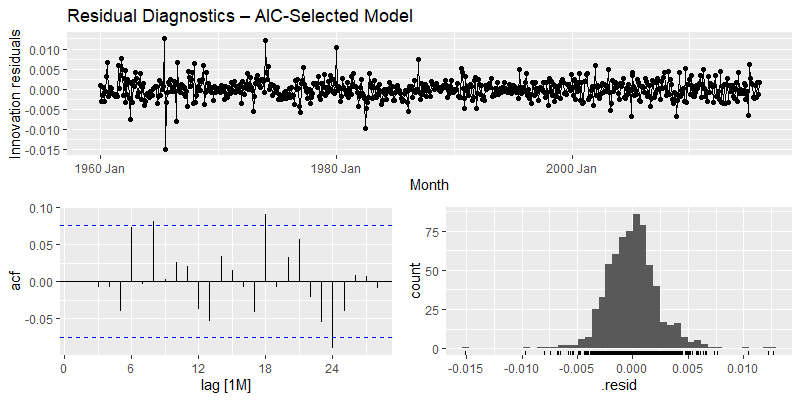
\includegraphics[width=0.7\linewidth]{billeder/Residual_Diagnostics_AIC.png}
    \caption{Residuals over time (top), ACF of residuals (bottom left) and distribution of residuals}
    \label{fig:placeholder}
\end{figure}


\section{Forecasting and Accuracy}

We produce 48-month ahead forecasts (January 2016 -- December 2019) from both models in log scale, plotted with the actual test data and 95\% prediction intervals.

\textbf{Accuracy}: Table~\ref{tab:acc} shows that the manually identified model outperforms the AIC-selected model across all three accuracy measures.

\begin{table}[H]
\centering
\begin{tabular}{lccc}
\hline
Model & RMSE & MAE & MAPE (\%) \\
\hline
AIC-selected                       & 0.0258 & 0.0207 & 0.446 \\
Manual ARIMA$(1,1,1)(0,1,1)[12]$   & 0.0186 & 0.0149 & 0.322 \\
\hline
\end{tabular}
\caption{Forecast accuracy on the test set (Jan 2016 -- Dec 2019), in log scale.}
\label{tab:acc}
\end{table}

\textbf{Discussion}: Although the AIC-selected model fits the training data better, the manually identified ARIMA$(1,1,1)(0,1,1)[12]$ generalises better out of sample, with RMSE, MAE, and MAPE significantly lower. This reflects that a complex model can overfit patterns in the training data that do not persist in new observations. The result also validates the model identification in Section \ref{Question 1.4} — the ACF/PACF analysis pointed to ARIMA$(1,1,1)(0,1,1)[12]$ as a natural fit, and the out-of-sample evaluation confirms it.

\begin{figure}[H]
    \centering
    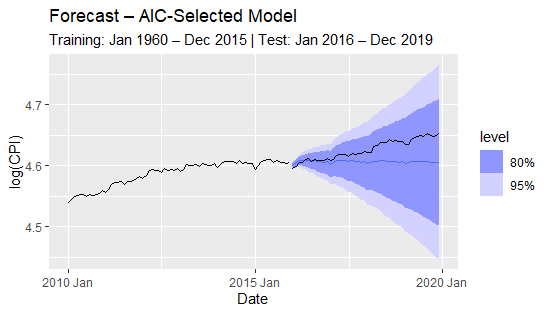
\includegraphics[width=0.45\textwidth]{billeder/Forecast_AIC.png}
    \hspace{1cm}
    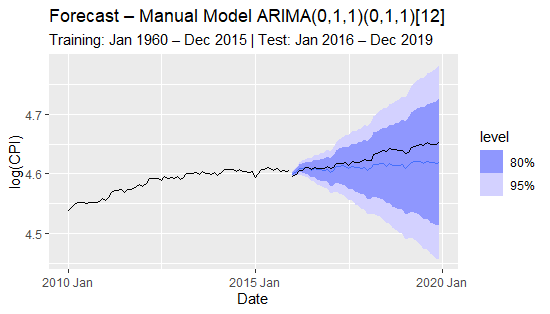
\includegraphics[width=0.45\textwidth]{billeder/Forecast_Manual.png}
    \caption{48-month forecasts for the AIC-selected (left) and manual ARIMA$(1,1,1)(0,1,1)[12]$ (right) models, with 80\% and 95\% prediction intervals. Black line: actual test data.}
    \label{fig:forecasts}
\end{figure}